\documentclass{patmorin}
\setlength{\parskip}{1ex}
\listfiles
\usepackage{pat}
\usepackage{paralist}
\usepackage{dsfont}  % for \mathds{A}
\usepackage[utf8x]{inputenc}
\usepackage{skull}
\usepackage{paralist}
\usepackage{graphicx}
\usepackage[noend]{algorithmic}

\usepackage[normalem]{ulem}
\usepackage{cancel}
\usepackage{enumitem}

\usepackage{todonotes}

\usepackage[longnamesfirst,numbers,sort&compress]{natbib}

% \usepackage[mathlines]{lineno}
% \setlength{\linenumbersep}{2em}
% \linenumbers
% \rightlinenumbers
% \linenumbers
% \newcommand*\patchAmsMathEnvironmentForLineno[1]{%
%  \expandafter\let\csname old#1\expandafter\endcsname\csname #1\endcsname
%  \expandafter\let\csname oldend#1\expandafter\endcsname\csname end#1\endcsname
%  \renewenvironment{#1}%
%     {\linenomath\csname old#1\endcsname}%
%     {\csname oldend#1\endcsname\endlinenomath}}%
% \newcommand*\patchBothAmsMathEnvironmentsForLineno[1]{%
%  \patchAmsMathEnvironmentForLineno{#1}%
%  \patchAmsMathEnvironmentForLineno{#1*}}%
% \AtBeginDocument{%
% \patchBothAmsMathEnvironmentsForLineno{equation}%
% \patchBothAmsMathEnvironmentsForLineno{align}%
% \patchBothAmsMathEnvironmentsForLineno{flalign}%
% \patchBothAmsMathEnvironmentsForLineno{alignat}%
% \patchBothAmsMathEnvironmentsForLineno{gather}%
% \patchBothAmsMathEnvironmentsForLineno{multline}%
% }


\newcommand{\coloured}[2]{{\color{#1}{#2}}}
\newenvironment{colourblock}[1]{\color{#1}}{}

% Taken from
% https://tex.stackexchange.com/questions/42726/align-but-show-one-equation-number-at-the-end
\newcommand\numberthis{\addtocounter{equation}{1}\tag{\theequation}}




\title{\MakeUppercase{Notes on Distance Labelling of Unweighted Planar Graphs}\thanks{This research was partly funded by NSERC.}}
\author{Pat Morin%
    \thanks{School of Computer Science, Carleton University}}


\DeclareMathOperator{\dist}{dist}
\DeclareMathOperator{\depth}{depth}
\DeclareMathOperator{\polylog}{polylog}
\DeclareMathOperator{\diam}{diam}

\newcommand{\comparable}{\mathbin{\diamond}}


\newcommand{\colored}[2]{{\color{#1}#2}}

\usepackage{tabularx}


\begin{document}

% \begin{titlepage}
\maketitle

\begin{abstract}
    These are some notes on ideas for a distance labelling scheme for planar graphs.
    % We give a \emph{distance labelling scheme} for unweighted undirected planar graphs in which each vertex is assigned a label of length $O(n^{1/3}\polylog n)$ such that the labels of any two vertices are sufficient to compute the distance between them.
\end{abstract}

\section{Introduction}

A class of $\mathcal{G}$ of graphs has an $f(n)$-bit \emph{distance labelling scheme} if there exists a function $D:\{0,1\}^*\to\N$ such that, for each $n$-vertex graph $G\in\mathcal{G}$ there exists a \emph{labelling} $\varphi_G:V(G)\to\{0,1\}^{f(n)}$ such that $D(\varphi_G(v),\varphi_G(w)) = \dist_G(v,w)$ for each pair of vertices $v,w\in V(G)$.

\begin{thm}\label{main}
    The class of planar graphs has an $O(n^{1/3}\polylog n)$-bit distance labelling scheme.
\end{thm}

\section{The Main Tool}
\label{main_tool}
really
Let $G$ be a graph.\footnote{All graphs are connected, finite, undirected, simple, and unweighted, unless specified otherwise}  For any $x,y\in V(G)$, let $\dist_G(x,y)$ denote the minimum length of a path in $G$ with endpoints $x$ and $y$.  Any path $x_1,\ldots,x_m$ of length $\dist_G(x_1,x_m)$ is called an $(x_1,x_m)$ \emph{$G$-geodesic}.

Let $T$ be a rooted tree.  A node $x\in V(T)$ is a \emph{$T$-ancestor} of $y\in V(T)$ if $x=y$ or $x$ is a $T$-ancestor of the parent of $y$.  If $x$ is a $T$-ancestor of $y$, then $y$ is a \emph{$T$-descendant} of $x$.  Note that every node of $T$ is both a $T$-ancestor and $T$-descendant of itself.  We use $\preceq_T$ to denote the $T$-ancestor relationship.  If $x\prec_T y$ and $x\neq y$ then we say that $x$ is \emph{strict} $T$-ancestor of $y$, $y$ is a \emph{strict} $T$-descendant of $x$ and $\prec_T$ denotes the partial order over $V(T)$ defined by the strict $T$-ancestor relation.  Define the relation $\comparable_T$ such that $x\comparable_T y$ if and only if $x\preceq_T y$ or $y\preceq_T x$.

For two nodes $x,y\in V(T)$, $P_T(x,y)$ denotes the unique path from $x$ to $y$ in $T$.  A path $v_1,\ldots,v_{m}$ in a rooted tree $T$ is \emph{$T$-downward} $v_1\preceq_T v_m$, is \emph{$T$-upward} if $v_m\preceq_T v_1$ and is \emph{$T$-vertical} if it is upward or downward.



\subsection{When $v_1$ and $w_1$ are on the same face}

Let $G$ be a plane graph, let $T$ be a BFS tree of $G$, and let $v_1,\ldots,v_s$ and $w_1,\ldots,w_t$ be disjoint upward paths in $T$ with $v_1$ and $w_1$ on the same face of $G$.  We are interested labelling $v_1,\ldots,v_s$ and $w_1,\ldots,w_t$ so that we can recover $\dist_G(v_i,w_j)$ from the labels of $v_i$ and $w_j$ for any $i,j\in\{1,\ldots,s\}\times\{1,\ldots,t\}$.


% First observe that this is trivial to achieve using $O(\log n)$-bit labels if  $v_1\comparable_T w_1$ since then all vertices are contained in a single vertical path in $T$.  Since $T$ is a BFS tree, this implies that $\dist_G(v_i,w_j)=|\depth_T(v_i)-\depth_T(w_j)|$.
%
% Now we consider the interesting case in which neither of $v_1$ or $w_1$ is a $T$-ancestor of the other.

Let $a$ be the lowest-common $T$-ancestor of $v_s$ and $w_t$.  Since $v_1$ and $w_1$ are on the same face of $G$, there exists a Jordan curve $f$ that contains every edge of $P_T(v_1,w_1)$, but does not intersect the interior of any other edge of $G$.  Let $f_0$ and $f_1$ be the two components of $\R^2\setminus f$.  For each $b\in\{0,1\}$, let $G_b$ be the subgraph of $G$ containing every edge and vertex of $G$ contained in $f\cup f_b$.

\begin{obs}\label{in_out}
    For any $i,j\in\{1,\ldots,s\}\times\{1,\ldots,t\}$,  $\dist_G(v_i,w_j)=\min\{\dist_{G_b}(v_i,w_j): b\in\{0,1\}\}$.
\end{obs}

\begin{proof}
    Let $a$ be the lowest common $T$-ancestor of $v_1$ and $w_1$. If $P$ is a $G$-geodesic that begins at $v_i$ and ends at $w_j$ that contains a vertex $x\in f_0$ and a vertex $z\in f_1$, then $P$ contains a vertex $y\in f$.  If $y\in V(P_T(a,v_1))$, then portion of $P$ from $v_i$ to $y$ can be replaced with $P_T(v_i,y)$ without increasing its length.  If $y\in V(P_T(a,w_1))$ then the portion of $P$ from $y$ to $w_j$ can be replaced with $P_T(y,w_j)$ without increasing its length.  In either case, the resulting geodesic has fewer vertices in $f_0\cup f_1$. Since $P$ is finite we can therefore repeat this until $P$ has no vertices in $f_0$ or $P$ has no vertices in $f_1$.
\end{proof}

B \cref{in_out} it suffices to focus on labels that allow us to recover $\dist_{G_b}(v_i,w_j)$ for each $b\in\{0,1\}$.  For concreteness, we focus on the case $b=0$. The case $b=1$ is handled identically.

Let $M$ be the $s\times t$ distance matrix in which $M_{i,j}:=\dist_{G_0}(v_i,w_j)$ for each $i,j\in\{1,\ldots,s\}\times\{1,\ldots,t\}$.  \citet{abboud.gawrychowski.ea:near-optimal} observe that, because $v_1,\ldots,v_s$ and $w_1,\ldots,w_t$ are on a common face of $G_0$,  $M$ has the following \emph{unit Monge property}:
\begin{compactenum}[(UM1)]
    \item For each $i,j\in\{2,\ldots,s\}\times\{1,\ldots,t\}$, $M_{i,j}-M_{i-1,j} \in \{-1,0,1\}$.\label{unit_property1}
    \item For each $i,j\in\{1,\ldots,s-1\}\times\{1,\ldots,t-1\}$, $M_{i,j}+M_{i+1,j+1} \le M_{i+1,j} + M_{i,j+1}$.\label{monge_property}
\end{compactenum}

Let $S$ be the $s\times t$ matrix defined by
\begin{equation}
    S_{i,j}=\begin{cases}
                0 & \text{if $i=1$} \\
                M_{i,j}-M_{i-1,j} & \text{otherwise}
            \end{cases}  \label{s_definition}
\end{equation}
It follows from \cref{unit_property1,monge_property} that each row $S_{i,*}$ of $S$ is non-increasing and contains only entries from $\{-1,0,1\}$, i.e., $1\ge S_{i,1}\ge S_{i,2}\ge\cdots\ge S_{i,t}\ge -1$. In particular, any row of $S_i$ can be encoded in $O(\log t)$ bits by storing the index of the first $0$ and the first $-1$.  More precisely, by defining  $j_{i,0}:=\min\{0\}\cup\{j\in\{1,\ldots,t\}:S_{i,j}=0\}$ and $j_{i,-1}:=\min\{t+1\}\cup\{j\in\{1,\ldots,t\}:S_{i,j}=-1\}$ we get
\[
    S_{i,j} = \begin{cases}
        1 & \text{if $j < j_{i,0}$} \\
        0 & \text{if $j_{i,0}\le j < j_{i,-1}$} \\
        -1 & \text{if $j_{i,-1}\le j$.}
    \end{cases}
\]

Observe that, for any $1\le i_0\le i\le s$ and any $j\in\{1,\ldots,t\}$,
\begin{equation}\label{recovery}
   M_{i,j} = M_{i_0,j} + \sum_{i'=i_0+1}^i (M_{i',j}-M_{i'-1,j}) = M_{i_0,j} + \sum_{i'=i_0+1}^i S_{i,j} \enspace .
\end{equation}


This suggests a distance labelling scheme that partitions $M$ in blocks consisting of $\ell$ consecutive rows, for some integer $\ell$.  In this scheme, $w_j$ stores $M_{i_0,j}$ for each $i_0\in I := \{1,1+\ell,1+2\ell,\ldots,1+\floor{(s-1)/\ell}\}$ and $v_i$ stores $S_{i_0+1,*},\ldots,S_{i,*}$ for $i_0=\max I\cap\{1,\ldots,i\}$.  It is straightforward to check that the labels of $v_i$ and $w_j$ contain all the information needed to evaluate \cref{recovery} and recover $M_{i,j}=\dist_G(v_i,w_j)$.

With this scheme, the label of $v_i$ has length $O((i-i_0)\log t)\subseteq O(\ell\log t)\subseteq O(\ell\log n)$ and the label of $w_j$ has length $O((s/\ell)\log n)$.

\begin{lem}\label{sameface_labelling}
    Let $\ell$ be a positive integer, let $G$ be an $n$-vertex plane graph, let $T$ be a BFS tree and let $v_1,\ldots,v_s$ and $w_1,\ldots,w_t$ be two disjoint upward paths in $T$ in which $v_1$ and $w_1$ are on a common face of $G$.    Then there exists an assignment of $O((\ell + s/\ell)\log n)$-bit labels to $v_1,\ldots,v_s$ and $w_1,\ldots,w_t$ such that $\dist_G(v_i,w_j)$ can be computed from the labels of $v_i$ and $w_j$, for any $i,j\in\{1,\ldots,s\}\times\{1,\ldots,t\}$.\todo{Formalize this with the notion of partial labelling scheme.}
\end{lem}

The optimal choice of $\ell$, in this case, is $\ell=\Theta(\sqrt{s})$ which gives a scheme using labels of length $O(\sqrt{s}\log n)$.  Of course, this is not yet enough to obtain an efficient general scheme for planar graphs.  Note that there is a symmetry between the two paths $v_1,\ldots,v_s$ and $w_1,\ldots,w_t$, so we may assume that $s\le t$.


\subsection{When $v_1$ and $w_1$ are not on the same face}

Next we extend the labelling scheme in the previous section so that it works when the vertices $v_1$ and $w_1$ are not on the same face.  This extension is not immediate because there is obvious choice for the Jordan curve $f$ that defines $G_0$ and $G_1$.

A path $x_1,\ldots,x_k$ in $G$ is \emph{$T$-conforming} if, for each $1\le i< j\le k$ such that $x_i\comparable_T x_j$, the subpath $x_i,\ldots,x_j$ is $T$-vertical.

\begin{obs}\label{conforming_geodesic}
    For any graph $G$, any BFS tree $T$ of $G$, and any $x,y\in V(G)$, there exists a $T$-conforming $(x,y)$ $G$-geodesic.
\end{obs}

Let $P:=P_T(v_1,w_1)$ and let $X$ be a $T$-conforming $G$-geodesic from $v_1$ to $w_1$.  If $X=P$, then the problem is trivial, since $\dist_G(v_i,w_j)=\dist_{X}(v_i,w_j)$ and a labelling that simply numbers the vertices according to their position in $X$ is sufficient.

If $X\neq P$ then the graph $P\cup X$ has two faces $f_0$ and $f_1$ whose boundaries intersect in a cycle $f$.  Although this looks like the previous case, we are not quite done.  \cref{in_out} does not hold for this definition of $f$, $f_0$, and $f_1$.  In particular, there may exist $v_i$ and $w_j$ such that every $G$-geodesic from $v_i$ to $w_j$ contains a vertex in $f_0$ and a vertex in $f_1$.   We now examine how this happens.

By \cref{conforming_geodesic}, there exists a geodesic $P_{ij}:=x_1,\ldots,x_k$ with $x_1=v_i$ and $x_2=w_j$.  By definition $P_{ij}\cap P_T(a,v_1)$ and $P_{ij}\cap P_T(a,w_1)$ are each paths.  Using the same strategy used in the proof of \cref{in_out} we can also guarantee that $P_{ij}\cap X$ is either empty or a path.  When $P_{ij}\cap X$ is empty, $P_{ij}$ is contained in $G_b$ for some $b\in\{0,1\}$, and we have already given a labelling scheme that allows us to compute $\dist_{G_b}(v_i,w_j)$.

To handle cases where $P_{ij}\cap X$ is not empty, we define $\dist'(v_i,w_j)$ as the length of the shortest path from $v_i$ to $w_j$ that contains at least one vertex of $X$, i.e., $\dist'(v_i,w_j):=\min\{\dist_G(v_i,x)+\dist_G(w_j,x): x\in V(X)\}$.  The preceding discussion is essentially a proof of:

\begin{obs}\label{in_out2}
    For any $i,j\in\{1,\ldots,s\}\times\{1,\ldots,t\}$,  $\dist_G(v_i,w_j)=\min\{\dist'(v_i,w_j)\cup\{\dist_{G_b}(v_i,w_j): b\in\{0,1\}\}$.
\end{obs}

Let $M'$ be the distance matrix defined by $\dist'$, so that $M'_{i,j}:=\dist'(v_i,w_j)$.  The matrix $M'$ certainly has the unit property (UM\ref{unit_property1}).  It also has a the Monge property (UM\ref{monge_property}), except that the inequality is reversed:  $M'_{i,j}+M'_{i+1,j+1} \ge M'_{i+1,j}+M'_{i,j+1}$.\todo{This is not quite right, strange things happen when $X$ contains edges of $T$.}  This reversal does not prevent us from applying the same labelling scheme.  In fact, the only difference is that the matrix $S'$ defined analogously to $S$ has rows that are non-decreasing rather than non-increasing.  This proves the following result:


\begin{lem}\label{general_labelling}
    Let $\ell$ be a positive integer, let $G$ be an $n$-vertex planar graph, let $T$ be a BFS tree and let $v_1,\ldots,v_s$ and $w_1,\ldots,w_t$ be two disjoint upward paths in $T$. Then there exists an assignment of $O((\ell + s/\ell)\log n)$-bit labels to $v_1,\ldots,v_s$ and $w_1,\ldots,w_t$ such that $\dist_G(v_i,w_j)$ can be computed from the labels of $v_i$ and $w_j$, for any $i,j\in\{1,\ldots,s\}\times\{1,\ldots,t\}$.\todo{Formalize this with the notion of partial labelling scheme.}
\end{lem}

\todo[inline]{This generalizes to any two vertex disjoint geodesic.  Make a ``2-connected'' graph by joining endpoints of the input geodesics with (at most $4$) geodesic edges.  Call these geodesic edges $e_1,\ldots,e_k$.  Then consider all $\sum_{j=0}^k j!$ sequences of edges that a shortest path from $v_i$ to $w_j$ might cross. (These are what is called homotopy classes, I think.)}

\subsection{Geodesic versus everyone}

Next we show how to extend \cref{sameface_labelling} so that we can compute $\dist_G(v_i,z)$ for any vertex $z\in V(G)$.


The setting is the following $v$ and $w$ are vertices on the same face of $G$, $a$ is the lowest common $T$-ancestor of $v$ and $w$, $s:=\dist_G(a,v)=\depth_T(v)-\depth_T(a)$, and $\depth_T(w)-\depth_T(v)\in\{0,1\}$.  Let $v_1,\ldots,v_s:=P_T(v,a)$.  As before, we use the Jordan cycle $f$ that defines two graphs $G_0$ and $G_1$. We focus on assigning labels so that we can compute $\dist_{G_0}(v_i,x)$ for any $i\in\{1,\ldots,t\}$ and any $x\in V(G_0)$.  Assume, for now, that $G$ has no separating triangles.\todo{Deal with these later, via a separating triangle tree.}

For $x\in V(P_T(v,a))$, this is easy $\dist_{G_0}(v_i,x)=|\depth_T(x)-\depth_T(v_i)$.  Thus, a label of length $O(\log n)$ suffices.  For $x\in V(P_T(w,a))$, we can use \cref{sameface_labelling} to assign labels of length $O((\ell+s/\ell)\log n)$.  Thus, we need only consider the case where $x\in f_0$, i.e., $x\in V(G_0-P_T(v,w))$.  Let $t:=|V(G_0-P_T(v,w))|$

To do this, we want to define an $s\times t$ distance matrix that has the unit Monge property.  For each $x\in V(G_0)$ and each $i\in\{1,\ldots,s\}$, define
\[
    I_{x,i}:=\{j\in\{1,\ldots,s\}: \text{there exists a $G_0$-geodesic from $x$ to $v_i$ that contains $v_j$}\}
\]
Of course $i\in I_{x,i}$ since every $G_0$-geodesic from $x$ to $v_i$ contains $v_i$.  The following observation shows that $I_{x,i}$ is a contiguous set of integers:

\begin{obs}\label{contiguous}
    If $x\in V(G_0)$, $i\in\{1,\ldots,s\}$, and $I_{x,i}$, and integers $a <z <b$ such that $a,b\in I_{x,i}$ then $z\in I_{x,i}$.
\end{obs}

In light of \cref{contiguous}, we will define $a_{x,i}:=\min I_{x,i}$ and $b_{x,i}:=\max I_{x,i}$. The following lemma shows that $a_{x,i}$ and $b_{x,i}$ are monotone with respect to $i$.

\begin{obs}\label{monotone}
    For each $x\in V(G_0)$ and $i\in\{1,\ldots,s-1\}$, $a_{x,i} \le a_{x,i+1}$ and $b_{x,i}\le b_{x, i+1}$.
\end{obs}

Now we get to the Unit Monge Property we want:

\begin{obs}
    For each $x\in V(G_0)$ and $i\in\{1,\ldots,s-1\}$, $i\not in I_{x,i+1}$ or $i+1\not\in I_{x,i}$.
\end{obs}

\begin{proof}
    If $i\in I_{x,i+1}$, then $\dist_{G_0}(x,v_{i+1}) = \dist_{G_0}(x,v_i)+1 > \dist_{G_0}(x,v_i)$.  This implies that $\dist_{G_0}(x,v_{i+1})+\dist_{G_0}(v_{i+1},x)>\dist_{G_0}(x,v_i)$ so there is no $G_0$-geodesic from $x$ to $v_i$ that contains $v_{i+1}$, so $i+1\not\in I_{x,i}$.
\end{proof}












\section{Easy Stuff}

Let $G$ be an $n$-vertex planar graph and let $T$ be a BFS spanning tree of $G$. Define the partition $\mathcal{L}:=\{L_i: i\in\N\}$ where $L_i:=\{v\in V(G):\depth_T(v)=i\}$, for each $i\in \N$.  The partition $\mathcal{L}$ is called a \emph{BFS layering} of $G$.  Since $G$ is finite, there exists $h:=\max\{i\in\N:L_i\neq\emptyset\}$.

Let $C$ be a large constant and let let $I:=\{i\in\{1,\ldots,h\}: |L_i|\le Cn^{2/3}\}$.
Let $a:=\max\{i\in I: \sum_{i'=0}^i |L_{i'}| \le 2n/3\}$ and $b:=\min\{i\in I: \sum_{i'=i}^h |L_{i'}| \le 2n/3\}$.  We distinguish between three cases:
\begin{enumerate}
    \item $a \ge b$.  This case is easy to handle: Define the \emph{separator} $S:=L_{a}$ and observe that $G-S$ has no component larger than $2n/3$. Let $C_1,\ldots,C_k$ be the components of $G-S$.  For each $r\in\{1,\ldots,k\}$ and each $v\in V(C_r)$ the label $\varphi(v)$, of $v$ contains
    \begin{compactenum}
        \item the integer $r(v):=r$;
        \item the distance sequence $d(v):=\langle \dist(v,x): x\in L_a\rangle$; and
        \item a recursively-defined label $\varphi_1(v)$ obtained by recursing on $C_r$.
    \end{compactenum}
    To determine $\dist_G(v,w)$ given $\varphi(v)$ and $\varphi(w)$ there are two cases to consider:
    \begin{compactenum}
        \item $r(v)\neq r(w)$: In this case $S$ separates $v$ and $w$, so every path from $v$ to $w$ in $G$ contains a vertex in $S$.  In particular, there is some $(v,w)$ $G$-geodesic that contains some $x\in S$.  This implies that $\dist_G(v,w)=\min\{\dist_G(v,x)+\dist_G(w,x): x\in S\}$ and this can be computed from $d(v)$ and $d(w)$.

        \item $r:=v(v)=r(w)$.  In this case, there is a $(v,w)$ $G$-geodesic  that is contained in $C_r$, or every $(v,w)$ $G$-geodesic contains a vertex of $S$.  Therefore, $\dist_G(v,w)=\min\{\dist_{C_r}(v,w)\}\cup \{\dist_G(v,x)+\dist_G(w,x): x\in S\}$.  The first quantity in this union can be computed from $\varphi_1(v)$ and $\varphi_1(w)$. The second quantity can be computed as described above.
    \end{compactenum}

    \item $0 < b-a \le Cn^{1/3}$.  In this case, we define $S:=L_a\cup L_b\cup X$ where $X\subseteq \bigcup_{i=a+1}^{b-1}$ consists of $2$ vertical paths in $T$ such that $G-S$ has no component of size larger than $2n/3$.  The existence of such a set $X$ is implicit in the work of \citet{lipton.tarjan:applications} and is treated explicitly by \citet{dujmovic:graph}.  We then proceed exactly as in the previous case.

    \item $b-a > Cn^{1/3}$.  In this case, we let $S:=L_a\cup L_b$ and proceed as in Case~1 except that one of the components of $G-S$ contained in $G[\bigcup_{i=a+1}^{b-1}L_i]$ may have size greater than $2n/3$.  We must treat this component differently.

    Let $G_{ab}:=G[\bigcup_{i=a}^b L_i]$.  Since $|L_i|\ge Cn^{1/3}$ for each $i\in\{a+1,\ldots,b-1\}$, $b-a-1\le n^{2/3}/C$.  This is important, because it means that $G_{ab}$ has a layering using $n^{2/3}$ layers.  In particular, the separator $X$ defined in the previous case has at most  $2n^{2/3}/C$ vertices.  Using \cref{sameface_labelling}, we can therefore assign labels to vertices in $X$ of length $O(n^{1/3})$ so that we can compute $\dist_{G_{ab}}(v,w)$ for any $v,w\in X$.\todo{A bit more explanation here.}

    ``All'' that remains is to show that we can extend this to a labelling of all the vertices in $G_{ab}$ so that, for any $v,w\in G_{ab}$, we can compute $\min\{\dist_{G_{ab}}(v,x)+\dist_{G_{ab}}(x,w): x\in X\}$.  Holy shit this sounds impossible.  As a first step, let's just try to assign labels so that we can compute $\dist_{G_{ab}}(v,x)$ for any $v\in V(G_{ab})$ and any $x\in X$.
\end{enumerate}

The current plan is to show that, If $v_1,\ldots,v_k$ are vertices of $G_{ab}$ and we can't concisely represent $(\dist_{G_{ab}}(v_{k+1},x):x\in X)$ using combinations of $O(n^{1/3})$ intervals from $\{(\dist_{G_{ab}}(v_{i},x):x\in X):i\in\{1,\ldots,\}\}$ then the shortest path tree $T_{k+1}$ from $v_{k+1}$ to $X$ contains $\Omega(n^{2/3})$ edges that are not in any of the shortest path trees $T_1,\ldots,T_k$.  Let's start simple.

Let $G_{ab}'$ be one of the components of $G_{ab}-X$ and let $G_0:=G[V(G'_{ab})\cup V(X)]$.  Let $P$ and $Q$ be the two upward paths in $T$ that define $X$.  Let $M$ be the two distance matrices indexed by $V(G_{ab})\times V(P)$ and $V(G_{ab})\times Q$, respectively, where the columns of $M$ and $N$ are ordered in the same order that vertices appear in $P$ and $Q$.

We focus on $M$ and $P$, though everything we do next applies also to $N$ and $Q$.  It will be helpful for shortest paths in $G$ to be uniquely defined, and to prefer edges of $P$ over other edges in $G_0$.  To achieve both these goals, define $\epsilon := \tfrac{1}{2n^2}$, assign each edge $e$ of $P$ a generic weight $w_e$ in the interval $[1,1+\epsilon]$, and define each edge in $E(G_0)\setminus E(P)$ a generic weight $w_e$ in the interval $(1+\epsilon,1+2\epsilon)$.  In this context, generic simply means that, for any two disjoint sets $I,J\subseteq E(G_0)$, $\sum_{e\in I}w_e\neq \sum_{e\in J}w_e$.  For any two vertices $v,w$ of $G_0$, let $P_{vw}$ be the unique shortest path from $v$ to $w$ in this weighted graph.  Then
\begin{inparaenum}[(i)]
    \item for any $v,w\in V(G_0)$, $P_{vw}$ is a $(v,w)$ $G_0$ geodesic;
    \item for any $v,w\in V(G_0)$, $P_{vw}$ maximizes the number of edges of $P$ over all $(v,w)$ $G_0$-geodesics;
    \item for any $v,w,x,y\in V(G_0)$ $P_{vw}\cap P_{xy}$ is a $G_0$ geodesic.
\end{inparaenum}

Let $w$ be any vertex of $G_0$ and let $C:=M_{*,w}$ be the column vector in $M$ that lists the distances from $w$ to $v_1,\ldots,v_s:=P$, so $C_i:=M_{v_i,w}=\dist_{G_0}(v_i,w)$.   Since the edge $v_iv_{i+1}$ is in $G_0$, $C_i-C_{i+1}\in\{-1,0,1\}$, for each $i\in\{1,\ldots,s-1\}$.  Our goal is to assign labels to $V(G_0)$ so that, given the labels of $w$ and $v_i$ we can recover $\dist_{G_0}(v_i,w)=C_i$.

Let $T_w:=\bigcup_{i=1}^s P_{wv_i}$ be the shortest path tree from $w$ to $V(P)$.  Define the tree $T'_w$ by starting with $T_w$ and removing any vertex $v_i\in V(P)$ whose $T_w$-parent is also in $P$.  The number, $k$, of leaves in $T'_w$ is a useful measure of the complexity of $C_i$:

\begin{lem}
    If $T'_w$ has $k$ leaves, then $C_i$ has a representation using $O(k\log n)$ bits.
\end{lem}

\begin{proof}
    Let $I:=\{i\in\{1,\ldots,s\}: v_i\in V(T'_w)\}$. Label the elements of $I:=\{i_1,\ldots,i_k\}$ so that $i_1<i_2<\cdots<i_k$.  The representation of $C_i$ consists of the value $k$ (encoded using $O(\log n)$ bits) followed by the values $i_1,\ldots,i_k$ (encoded using $O(k\log n)$ bits), followed by the values $C_{i_1},\ldots,C_{i,k}$ (encoded using $O(k\log n)$ bits).

    For convenience, define $i_0=0$, $i_{k+1}=s+1$, and $C_{0}=C_{s+1}=\infty$.
    Given this encoding, to determine $C_i$ we find the unique $j\in\{0,\ldots,t\}$ such that $i_j\le i\le i_{j+1}$ and return $\min\{i-C_{i_j}, C_{i_{j+1}}-i\}$.
\end{proof}

% The following is not true.  We can make $T'_w$ a complete binary tree with $k$ leaves and subdivide each edge e 2^{log k - depth(e)} times.  The resulting tree has only $O(k\log k)$ nodes.
% The number of leaves of $T'_w$ also gives a surprisingly large lower bound on the size of $T'_w$:
%
% \begin{lem}
%     If $T'_w$ has $k$ leaves then $|T'_w)|\in \Omega(k^2)$.
% \end{lem}

\begin{lem}\label{cyclically_unimodal}
    For any $w_1,w_2\in V(G_0)$ with $d:=\dist_{G_0}(w_1,w_2)$, there exists a cyclically unimodal\todo{Define cyclically unimodal} $s$-vector $v\in\{-d,\ldots,d\}^s$ such that $M_{*,w_1}=M_{*,w_2}+v$.
\end{lem}

At this point, I'm well and truly stuck.  I was hoping to maybe do something with ideas from computational geometry related to ham-sandwiches, and/or centerpoints, but have not had much progress. For every $v_i\in V(P)$ and $w\in V(G_0)$ there is a collection of $G_0$ geodesics that contain $v_i$ and $w$.  (Start with the shortest path tree  $T_{v_i}$ and keep only the vertices that have $w$ as a descendant or an ancestor.)

Update: The next plan:
\begin{enumerate}
    \item Prove a version of \cref{cyclically_unimodal} that looks like the following:  Let $C$ be a cycle in $G$ consisting of two vertical paths in a BFS tree of $G$.  This partitions $G$ into $G_0$ (inside) and $G_1$ (outside).  Let $B$ be a ball in $G_0$ centered at $v\in V(G_0)$ such that $G_0[B]$ has treewidth at most $t$.  Let $\vec{v}$ be the distances vector from $v$ to $V(G_1)$ with the vertices listed in clockwise order.  Let $\vec{u}$ be the distance vector from $u$ to $V(G_1)$ with vertices listed in the same order.  Then $\vec{v}-\vec{u}$ has representation complexity $\tilde{O}(t)$.

    \item Such a lemma would be helpful because a ball of treewidth $t$ is guaranteed to contains a subdivision of a $t\times t$ grid, so it has $\Omega(t^2)$ vertices.  The idea then is to take $t=n^{1/3}$, cover $G_0$ with $O(n/t^2)=O(n^{1/3})$ of these balls and have each vertex in $G_1$ store its distance to each ball center $v$ and have each vertex $u\in B$ store the difference vector $\vec{v}-\vec{u}$.  Of course, we have to make sure that no vertex is contained in too many of these balls, but that shouldn't be a big problem.
\end{enumerate}

% These things behave a bit like lines. For example, for every $v_i$ there is a "halving line" that contains $v_i$ (this is a root-to-leaf path in $T_{v_i}$ with at most half the tree to its left and half the tree to its right.)  The vertices in $G_0$ also behave a bit like they have some size.  (Think of $v_i$ as a light and the subtree of $T_{v_i}$ rooted at $w$ as the shadow of $w$; as $w$ moves further away from $v_i$ it's shadow gets smaller.)
%
% Let $L(v_i,w)$ be the set of nodes in the subtree of $T_{v_i}$ that are related to $w$.  It seems like it would be useful to find $w$, $i$, and $\ell$ $G_0$ such that $\bigcap_{j=i}^{i+\ell} v_j L(v_j,w)$ has size $k$ for some large value of $k$.  This would allows us to encode all $k\ell$ distances $\dist_{G_0}(v_j,w')$ by having each of the nodes involved store their distances to $w$.

\section{An $\tilde{O}(\sqrt{n})$ bound using crossing numbers?}

Here's an alternative strategy.  Let $M$ be a set of unordered pairs of vertices of $G$ and let $G_M$ be the graph with vertex set $V(G)$ and edge set $E(G_M)=M$.  We obtain drawing of $G_M$ by drawing each edge $vw$ using (a slight perturbation of) the shortest path from $v$ to $w$ in $G$.  By the crossing lemma, this drawing has $\Omega(|M|^3/n^2)$ pairs of crossings edges.  Each pair of crossing edges corresponds to a pair of shortest paths in $G$ with a common vertex and we can charge that pair to their common vertex.  When we do this, some vertex $v\in V(G)$ is charged $\Omega((|M|/n)^3)$ times.  This means $v$ is involved in this many crossing pairs and therefore there are at least $\Omega((|M|/n)^{3/2})$ pairs $(x,y)\in M$ such that the shortest path from $x$ to $y$ in $G$ contains $v$.  This means that there are $\Omega((|M|/n)^{3/2})$ entries in the distance matrix that can be stored by having each vertex remember its distance to $v$.

Let $M_0$ consist of the $|M_0|=\binom{n}{2}$ pairs of vertices in $G$.  Applying the above, we have each vertex remember its distance to $v$ and this takes care of $\Omega((|M_0|/n)^{3/2})=\Omega(n^{3/2})$ entries in the distance matrix.  We then form $M_1$ by removing these pairs from $M_0$ and repeat.  Let $m_k=|M_k|$, this leads to a recurrence of the form:
\[  m_k = m_{k-1} - (m_{k-1}/n)^{3/2} \]
with $m_0=\binom{n}{2}$.  This starts out well and continues to do so until $k=\sqrt{n}$, at which point $m_k\approx \tilde{O}(n^{1+\epsilon})$.  Then it becomes much less efficient.  Still, it's hopeful.

We may even be able to do this without using the crossing lemma.  If we could get down to a case where the average distance between a of vertices $v,w$ of $G$ is $\Omega(\sqrt{n})$ then the total length of all paths is $\Omega(n^{5/2})$, so some vertex is involved in $\Omega(n^{3/2})$ paths.

% Hold on now.  We already know what to do if we have a BFS layering in which every $n^{1/3}$ consecutive layers contains a layer of size at most $n^{1/3}$. We also know what to if we have a separator of size $n^{1/3}$.  Thus, we can assume that for each $v$ in $G$, the BFS layering of $v$ contains a set of $\Omega(n^{1/3})$ consecutive layers each of size at least $n^{1/3}$ and whose total size is at least $(1-\epsilon)n$.  If I could show that the distribution over these layers is fairly uniform, then I would get an average distance of $\Omega(n^{1/3})$.

Here's an idea: Since $G$ has no $n^{1/3}$ separator, its treewidth is at least $n^{1/3}$, so it contains a subdivision of a $n^{1/3}\times n^{1/3}$ grid.  Since $G$ doesn't have any $n^{1/3}$ separator, I suspect one can strengthen that to say $G$ must contains a subdivision of an $n^{1/3}\times n^{2/3}$ grid.  This grid has $\Omega(n)$ vertices and average distance $\Omega(n^{2/3})$.  This makes the total distance $\Omega(n^{8/3})$ so, on average, each vertex can be used to cover $\Omega(n^{5/3})$ shortest paths.

% More usefully, in the product $G\subseteq H\boxtimes P$, $\diam(G)\ge\max\{\diam(P),\diam(H)\}$.  We already know $\diam(P)$ is large.  I think we can also figure out that $\diam(H)$ is large since, otherwise, we get a small separator.  So both $\diam(P)$ and $\diam(H)$ are large.
%
% is separated by at most $n^{1/3}$ layers of size greater than $n^{1/3}$, so we can assume we don't have one of those.  Therefore, for every $v\in V(G)$, the BFS layering of $G$ contains a

To gain some breathing room, we can always take $C n^{1/3}$ consecutive BFS layers and apply the naïve algorithm to the surrounding $3Cn^{1/3}$ layers.  This covers all paths between vertices in the middle layers that don't wander outside the two outer layers. In particular, it covers all paths of length at most $Cn^{1/3}$.  In fact we can do this as a first step to ensure that we don't have to worry about short paths at all.  We can also do this to the separator $X$ discussed above to reduce to a problem where we have two sets $A$ and $B$ separated by $n^{1/3}$ layers surrounding $X$ and we only have to worry about paths from $A$ to $B$.  The advantage of doing this on $X$ is that, since $X$ consists of two geodesics, any geodesic between $A$ and $B$ crosses $X$ only once.  So really it looks like the whole thing boils down to finding a solution for the bipartite ``well-separated'' case.

Can we use this kind of approach to beat $O(\sqrt{n})$-length labels?
Not without something more: Everything in here is also true about weighted graphs, so none of this can fully solve the problem.




% One very slack part of this argument comes from the fact that we only charge each pair of crossing paths for one of the vertices they have in common. I would guess that, on average, they have $\omega(1)$ vertices in common.  If an average pair had $\Omega(n^{1/3})$ vertices in common then we would get
% \[  m_1 = \binom{n}{2} - \Omega(n^{5/3}) \enspace . \]
% This is a great start, since it could lead to be done when $k=O(n^{1/3})$.




Some further avenues to explore:
\begin{enumerate}
    \item None of this uses the product structure theorem since it doesn't need to.  However, there's a subtle property of the connected path partition version of the theorem that seems relevant:  Any $G$-geodesic traces a simple path in the graph $H$.  This property comes from the fact that the parts of the partition $\mathcal{P}$ that define $H:=G/\mathcal{P}$ are themselves geodesics.  This seems like a very useful property.

    \item In the product structure $H\boxtimes P$, we know how to handle the case where $\diam(P)\in O(n^{1/3})$.  What about the case where $\diam(H)\in O(n^{1/3})$.  Does this imply that $G$ has small separators?  Answer, NO: If $H$ has any path of length $\omega(n^{1/3})$ then $H\boxtimes P$ contains a large grid so its treewidth is large.

\end{enumerate}


\section{The End?}

There's a family of bad examples involving a slight variation of a $d$-subdivision of a $d\times d$ grid.  In these examples, the distance vector from $v$ is unchanging, but there are $2^{d^2}$ distance vectors for $w$.  So just storing distances to $v$ doesn't help.  It also seems that just storing distances to $w$ doesn't help.  Finally, it doesn't look like storing distances to both $v$ and $w$ helps much when computing distances from $v$ to $w$.  On the other hand, this family of graphs has $O(d)=O(\sqrt[3]{n})$-sized separators\ldots

\begin{center}
    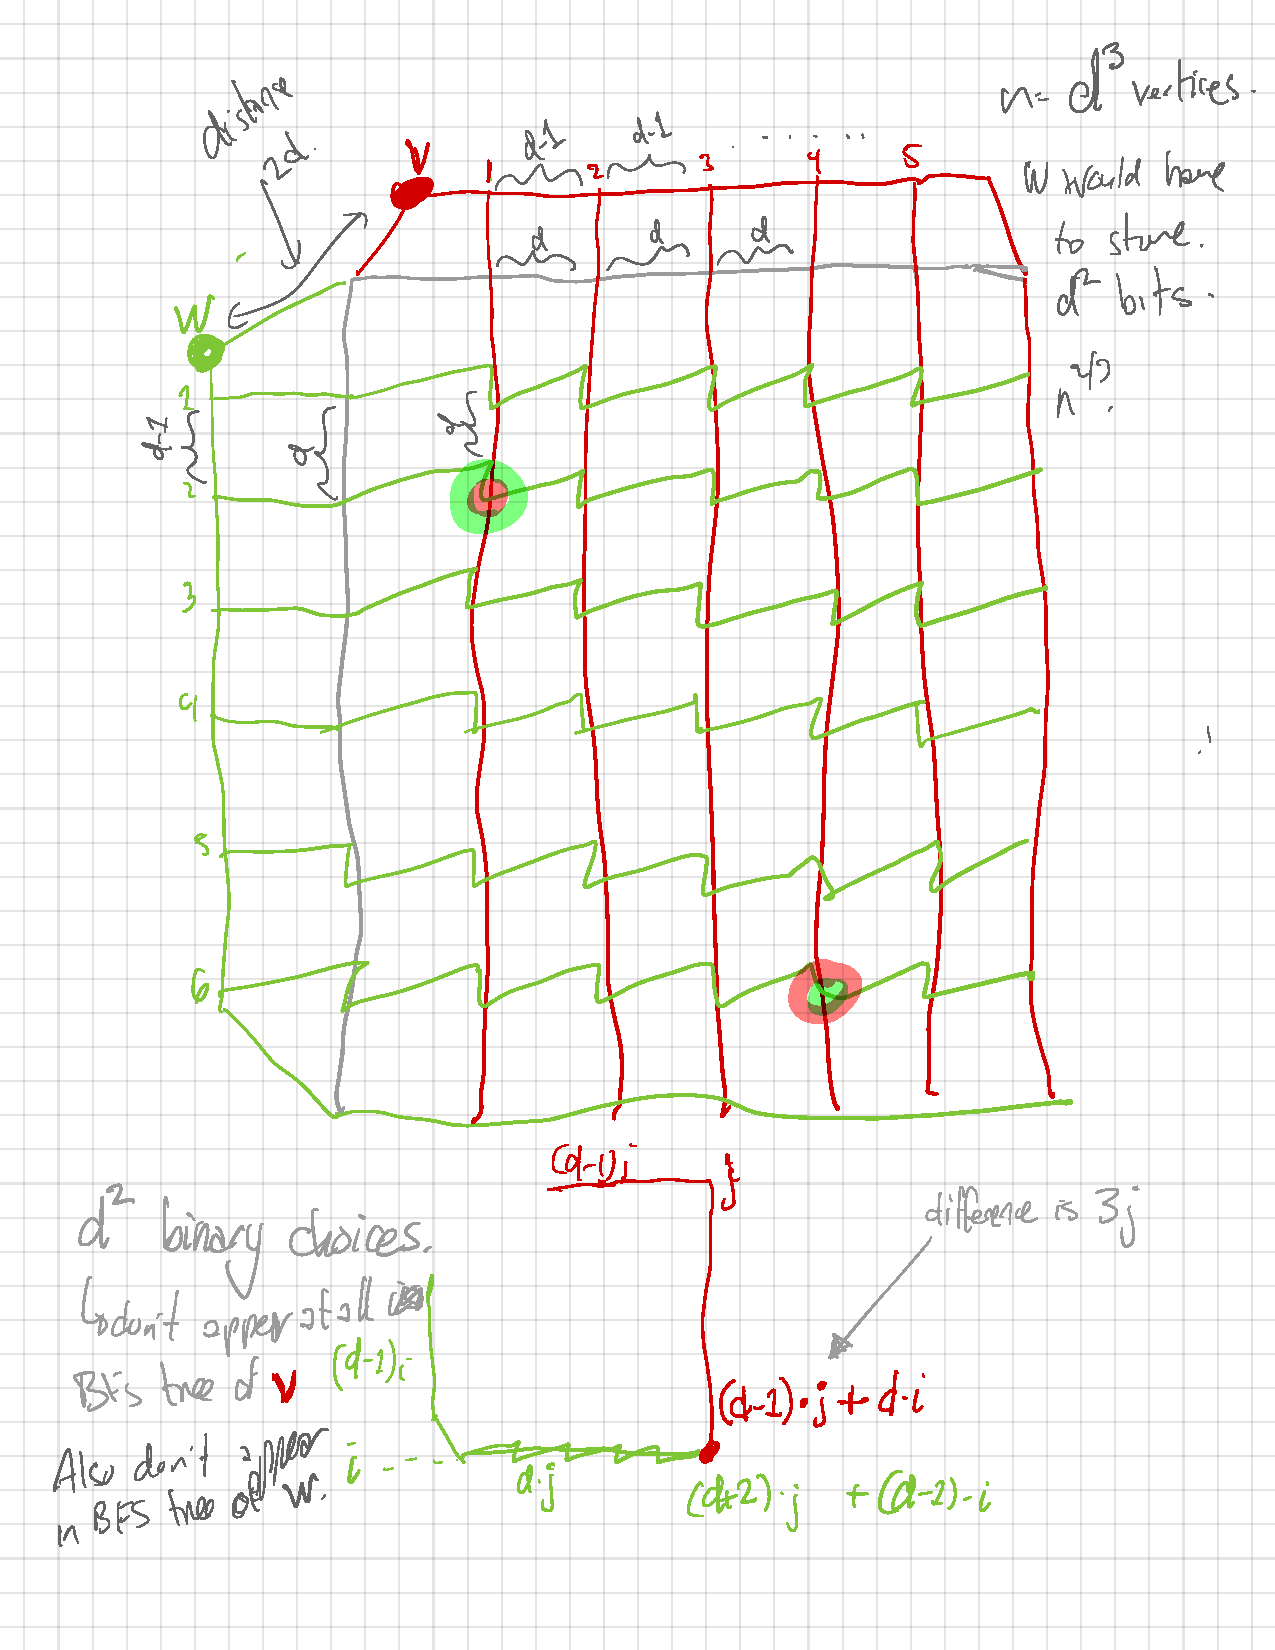
\includegraphics[width=.8\textwidth]{figs/bad-example}
\end{center}


\section{Connectivity Reductions}

In this section we describe a few tricks that can be used to reduce to more highly connected cases. Some of the ideas used might turn out to be be useful.

\subsection{Reduction to the Biconnected Case}

To reduce to the biconnected case, consider the \emph{block cut tree} $T$ of $G$.  This is a tree that indexes a sequence of subgraphs $(G_x:x\in V(T))$.
\begin{enumerate}
    \item For each cut vertex $v$ of $G$, $T$ contains a \emph{cut node} $x$ with $G_x:=(\{v\},\emptyset)$.
    \item For each biconnected component\footnote{A graph $G$ is \emph{biconnected} if $G-\{v\}$ is connected for any $v\in V(G)$.  A biconnected component of a graph $G$ is a maximal biconnected subgraph of $G$.} $C$ of $G$, $T$ contains a \emph{block node} $y$ with $G_y=C$.
    \item Any edge $xy$ is included in $T$ if and only if $x$ is a cut node, $y$ is a component node and $V(G_x)\subseteq V(G_y)$.
\end{enumerate}

The block cut tree $T$ contains a node $x^*$ such that $T-\{x^*\}$ has no component of size greater than $|T|/2$.\todo{We can save a log factor by using a weighted cut here instead}  Let $C$ be the set of components of $T-\{x^*\}$.  For each component $X\in C$, define the subgraph $G_X:=\bigcup_{x\in V(X)} G_x$ and the vertex $v_X$ as the unique element in the singleton set $V(G_X)\cap V(G_{x^*})$.  For each $w\in V(G)\setminus V(G_{x^*})$, let $X_w$ be the unique $X\in C$ such that $w\in V(X)$.


% For each vertex $v$ of $G_{x^*}$ define the subgraph
% \[
%     G_v = G\left[\{v\} \cup \cup\{V(X) : X\in C,\, v_X=v  \}
%     \right]
% \]

% Fix some constant $a$, $0<a < 1$, let $I:=\{X\in C: |G_v|\ge a |G|\}$, and let $\overline{I}:=V(G_{x^*})\setminus I$.  We call the elements of $I$ \emph{heavy vertices} of $G_{x^*}$ and the elements of $\overline{I}$ are the \emph{light vertices} of $G_{x^*}$.

We will show how to compute a distance labelling $\ell_G:V(G)\to\{0,1\}^*$ for the planar graph $G$ assuming we know how to compute a distance labelling for any biconnected planar graph.

If $|G|\le 1$ then the problem is trivial, so no labels are needed and $\ell_G(w):=\varepsilon$ for each $w\in V(G)$.  Otherwise, each vertex $w$ of $G$ is labelled with a label $\ell_G(w)$ that has the following parts:
\begin{compactenum}
    \item $\alpha(w):=x^*$
    \item $\beta(w)$, the unique vertex in $X_w\cap G_{x^*}$
    \item $\gamma(w):=\ell_{G_{x^*}}(\beta(w))$
    \item $\delta(w):=\dist_G(w,\beta(w))$
    \item $\epsilon(w):=X_w$\footnote{More precisely, $\epsilon(w)$ is a non-negative integer that identifies $X_w$, or $-1$ if $w\in G_{x^*}$.}
    \item $\zeta(w):=\ell_{G_{X_w}}(w)$ or $\zeta(w):=\varepsilon$ if $w\in V(G_{x^*})$
\end{compactenum}

Note that $\gamma(w)$ \emph{is not} recursively defined since $G_{x^*}$ is biconnected.  On the other hand $\zeta(w)$ \emph{is} recursively defined since $G_{\beta(w)}$ may not be biconnected.  Before analyzing the lengths of the labels in $\ell_G$, we first show how $\ell_G(v)$ and $\ell_G(w)$ can be used to compute $\dist_G(v,w)$.  We distinguish between the following cases:

\begin{compactenum}
    % \item If $\beta(v)=v$ and $\beta(w)=w$ then $v$ and $w$ are both vertices of $G_{x^*}$ and $\dist_G(v,w)=\dist_{G_{x^*}}(v,w)$ is computed using $\gamma(v)=\ell_{G_{x^*}}(v)$ and $\gamma(w)=\ell_{G_{x^*}}(w)$.

    % \item If $v':=\beta(v)=\beta(w)$ and $\epsilon(v)\neq\epsilon(w)$ then $\dist_G(v,w)=\dist_{G}(v,v')+\dist_G(v',w)$ is computed using $\delta(v)=\dist_G(v,v')$ and $\delta(w)=\dist_G(v',w)$.

    \item If $\beta(v)=\beta(w)$ and $X:=\epsilon(v)=\epsilon(w)$ then  $\dist_G(v,w)=\dist_{G_X}(v,w)$ is computed (inductively) using
     $\zeta(v)=\ell_{G_{X}}(v)$ and $\zeta(w)=\ell_{G_{X}}(w)$.

    % \item If $\beta(v)\in I$ then we can compute $\dist_G(v,w)=\dist_G(w,\beta(v))+\dist_G(\beta(v),v)$.  Since $\beta(v)\in I$, the first term can be obtained from $\epsilon(w)$.  The second term is $\delta(v)=\dist_G(\beta(v),v)$.

    % \item If $\beta(w)\in I$ then we proceed as in the previous case, reversing the roles of $v$ and $w$.

    \item Otherwise, $\dist_G(v,w)=\dist_{G}(v,\beta(v))+\dist_{G_{x^*}}(\beta(v),\beta(w))+ \dist_{G}(\beta(w),w)$. The first and last terms are computed using $\delta(v)=\dist_G(v,\beta(v))$ and $\delta(w)=\dist_G(\beta(w), w)$, respectively.  The middle term is computed from $\gamma(v)=\ell_{G_{x^*}}(\beta(v))$ and $\gamma(w)=\ell_{G_{x^*}}(\beta(w))$.
\end{compactenum}

Finally, we analyze the size of the resulting scheme.  Let $c$ be the exponent such that every $n$-vertex biconnected planar graph has a distance labelling scheme using labels of length $O(n^c)$.  Observe that $\ell_G(w)$ contains exactly one label $\gamma(w)$ from $\ell_{G_{x^*}}$ and this label has length $O(n^c)$.  The remaining parts $\ell_G(w)$ each have length $O(\log n)$ except for $\zeta(w)$, which is label from $\ell_{G_{X_w}}$.  The tree $X_w$ has size $|X_w|\le |T|/2$ and is the block cut tree for $G_{X_w}$.  Therefore, if $S(m)$ denotes the length of the longest label $\ell_G(w)$ obtained in an $n$-vertex planar graph $G$ whose block cut tree has $m$ nodes, then we obtain the recurrence
\[
  S(m) \le \begin{cases}
               O(n^c) & \text{if $m=1$} \\
               O(n^c) + S(m/2) &  \text{if $m>1$}
           \end{cases}
\]
which resolves to $S(m)=O(n^c\log m)$.\todo{See note before about shaving a log} Note that there is a subtlety here involving the vertices of $G_{x^*}$ These vertices may appear in $G_X$ for many components $X\in C$.  However, each such vertex $w$ does not receive (a) label(s) $\zeta(w)$.

\subsection{Reduction to the Triconnected Case}

For a reduction from the biconnected case to the triconnected case, we will try to proceed exactly as in the previous section, but instead of a block cut tree we use an SPQR-tree $T$.  In the previous case, we didn't make a distinction between the case where $x^*$ was a cut nodes or a block node, but here we do need to make a distinction between the different kinds of nodes in an SPQR-tree.

\begin{itemize}
    \item S nodes:  If $x^*$ is an S node then $G_{x^*}$ is a cycle that consists of viritual edges and real edges.  Each virtual edge $vw$ has a weight corresponding to the length of the shortest path from $v$ to $w$ in all of the graphs attached to $vw$.  To distance label $G_{x^*}$ we fix some vertex $v_0$ of $G_{x^*}$ and give each vertex $w$ a label consisting of the length of the cycle and the distance from $v_0$ clockwise around the cycle.  This makes it easy to compute $\dist_G(v,w)$ for any two vertices $v,w\in V(G_{})$

    \item P nodes: If $x^*$ is a P node then $G_{x^*}$ is a ``dipole graph'' with two vertices $v$ and $w$. In this case, we only care about the shortest path from $v$ to $w$.

    \item Q nodes: These are not really used.

    \item R nodes: If $x^*$ is an R node, then $G_{x^*}$ is a $3$-connected graph containing both real and virtual edges. Each virtual edge $vw$ is represented as weighted edge whose weight is equal to $\dist_G(v,w)$.  This result in a weighted 3-connected graph of total edge length $O(n)$.  By assumption, these can be labelled with labels of length $O(n^c)$.
\end{itemize}




\subsection{A General Solution}

More generally, we can always try to cut out subproblems






\bibliographystyle{plainurlnat}
\bibliography{distance-labelling}


\end{document}
